\documentclass[a4paper, 11pt]{article}

\usepackage{hyperref}
\voffset -0cm
\hoffset 0.0cm
\textheight 23cm
\textwidth 16cm
\topmargin 0.0cm
\oddsidemargin 0.0cm
\evensidemargin 0.0cm

\usepackage{epsfig}
\usepackage{setspace}
\usepackage{fancyheadings}
\usepackage{amsmath}
\usepackage{amssymb}
\usepackage{graphicx}
\usepackage{url}

\title{}
\author{}
\date{}

\begin{document}

\begin{center}
	\LARGE \textbf{TD12: Height maps and Mesh visualization}
\end{center}

\bigskip
\par In this TP, the objective is to practice a bit with triangular
mesh data-structures and 3D visualization using \texttt{DGtal}
viewer. The final objective is to render height maps as 3D meshes with
colorimetric information.

\section{Preliminaries}

Visualization will be performed by \texttt{DGtal}. If you use the
compiled library (``dcoeurjo'' account), the viewer is enabled by
default. If you use you own \texttt{DGtal} install, make sure that you
have compiled the library with \texttt{WITH\_QGLVIEWER} flag enables
(e.g. \texttt{cmake .. -DWITH\_QGLVIEWER=true}). You would need to
have Qt and QGLViewer installed in your system.

Please also checkout the last release of the \texttt{DGtalSkel} folder. The
file \texttt{image2mesh.cpp} gives examples of the \texttt{Viewer3D}
usage.

First, compile this example and when executing it, you should see an OpenGL
window with three triangles and two cubes.  For this TP, you just need
to know how to display triangles:
\begin{verbatim}
      Z3i::RealPoint p1(1.0,0.0,0.0),
        p2(0.0,1.0,0.0),
        p3(0.0,0.0,1.0);
      viewer.addTriangle(p1,p2,p3);
      viewer  << Viewer3D<>::updateDisplay;
\end{verbatim}


The idea is to construct a mesh from and image $I$ such that the mesh
vertices are given by 3D points $(i,j, I(i,j))$ for each point $(i,j)$
in the image domain.  As illustrated in Fig.~\ref{fig:image}, the mesh
is constructed from a regular pattern from alternate triangles with
respect to evenness of the x-coordinate for instance: $\{(i,j,I(i,j)),
(i+1,j,I(i+1,j)), (i,j+1,I(i,j+1))\}$ or $\{(i,j,I(i,j)),
(i+1,j-1,I(i+1,j-1)), (i+1,j,I(i+1,j))\}$

\begin{figure}[h]
  \begin{center}
    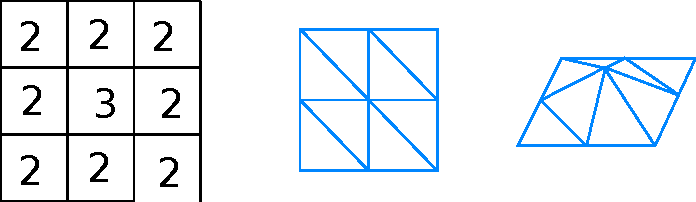
\includegraphics[width=10cm]{image2mesh}
  \end{center}
  \caption{Image to height map mesh.}
  \label{fig:image}
\end{figure}

Please note that \texttt{image2mesh.cpp} also illustrates the loading
of a PGM grayscale image.


\section{Mesh data-structure and visualization}

{\bf Question 1}  From a PGM image, construct a Face-Vertex data
structure: the Vertex array contains all point coordinates and the
Face array contains the set of faces (triple of vertex indices).


{\bf Question 2} Create a function which take in argument a mesh (the
two vectors) and send all triangles to a DGtal Viewer.



\section{Normal map rendering and curvature estimation}





\end{document}
